\bchapter{TensorFlow}
\section{Introduzione}
TensorFlow\cite{databricks} è una libreria open source per l'apprendimento automatico, il calcolo numerico e altre attività di analisi statistica e predittiva. Questo
tipo di tecnologia, sviluppata e rilasciata da Google nel novembre 2015, rende l’implementazione di modelli di machine learning più semplice e veloce per
gli sviluppatori, assistendoli nel processo di acquisizione dei dati, nella formulazione di previsioni su larga scala e nel successivo affinamento dei risultati.
Lo scopo principale di TensorFlow è la creazione e l’addestramento di reti neurali, che possono essere utilizzate per moltissime applicazioni\cite{egovaleo}, quali:
\begin{itemize}
    \item Classificazione delle immagini;
    \item Elaborazione del linguaggio naturale;
    \item Analisi delle serie temporali;
    \item Riconoscimento vocale;
    \item Sviluppo di soluzioni di visione artificiale;
    \item Ottimizzazione di chatbot;
    \item Sistemi di assistenza clienti automatizzati;
    \item Altri ancora.
\end{itemize}

La versatilità e il grande range di applicazioni rendono TensorFlow uno strumento veramente potente e, per questo, è il \textbf{motore di AI più utilizzato},
come si può osservare in figura \ref{fig:diagramma}.

\begin{figure}[ht]
    \centering
    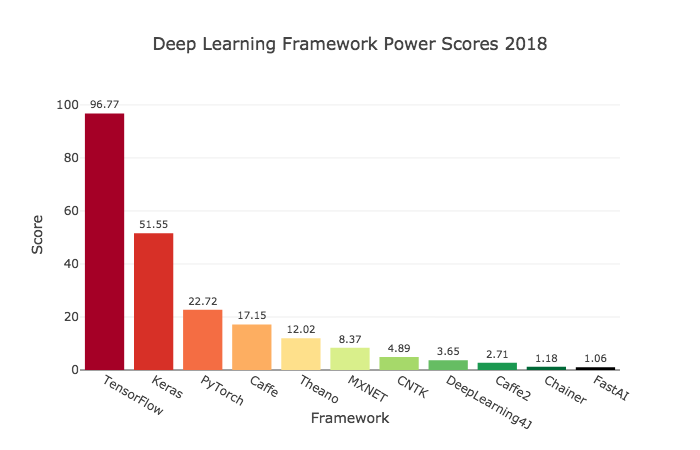
\includegraphics[width=0.8\textwidth]{Immagini/diagramma.png}
    \caption{Diagramma dei punteggi di utilizzo di vari framework nel 2018}
    \label{fig:diagramma}
\end{figure}

\section{TensorFlow Lite}
TensorFlow si può dire essere il “genitore” di TensorFlow Lite\cite{tensorflow}, introdotto da Google nel 2017, che non è altro che una versione ottimizzata per l’uso su
dispositivi embedded e mobili. TensorFlow Lite è un framework di deep learning open-source, che converte un modello TensorFlow pre-addestrato in un formato
specifico, che può essere ottimizzato per la velocità e l’archiviazione. Le sue caratteristiche principali sono:
\begin{itemize}
    \item Supporto per più piattaforme, coprendo dispositivi Android e iOS, Linux embedded e microcontrollori;
    \item Supporto per diversi linguaggi di programmazione, come Java, Swift, Objective-C, C++ e Python;
    \item Alte prestazioni, facendo ricorso all’accelerazione hardware e all’ottimizzazione del modello;
    \item Ottimizzato per l’apprendimento automatico sul dispositivo, affrontando 5 vincoli chiave:
 \begin{itemize}
        \item Latenza: TensorFlow Lite riesce ad eliminare il ritardo tra l’invio dei dati al server e il ricevimento della risposta. Infatti, il
        framework non necessita di inviare dati ad un server esterno (visto che l’apprendimento e l’elaborazione dei dati avvengono direttamente sul
        dispositivo) e, quindi, il tempo di predizione viene ridotto notevolmente;
        \item Privacy: è garantita la riservatezza massima nell’elaborazione di dati sensibili o personali che, infatti, non vengono mai condivisi con
        server remoti. Questo è possibile perché i dati non lasciano mai il dispositivo dell’utente, assicurando la massima privacy;
        \item Connettività: TensorFlow lite non necessita di una connessione internet permettendo lo svolgimento di attività di apprendimento e inferenza
        anche in situazioni in cui non è possibile o pratico avere una connessione stabile;
        \item Dimensioni del modello: i dispositivi mobili o embedded dispongono, generalmente, di risorse minori rispetto ai computer. La riduzione dello
        spazio di archiviazione e della necessità di risorse computazionali per un modello TensorFlow diventa, dunque, essenziale per l’esecuzione di
        algoritmi di Machine Learning sul dispositivo;
        \item Consumo energetico: l’elaborazione dei dati e l’inferenza di un modello di Machine Learning possono incidere pesantemente sulla durata della
        batteria di un dispositivo mobile. TensorFlow Lite, infatti, si occupa di gestire efficientemente il consumo di energia. Inoltre, l’eliminazione
        della necessità di trasmettere dati riduce ulteriormente il consumo energetico.
    \end{itemize}
\end{itemize}

\section{Workflow di sviluppo}
TensorFlow Lite, insieme a TensorFlow, offre tutti gli strumenti per la generazione e l’utilizzo di un modello di Machine Learning. Il workflow di
sviluppo è il seguente:
\begin{itemize}
    \item Generazione di un modello TensorFlow Lite: A questo scopo, si può decidere se utilizzare un modello di TensorFlow Lite esistente, creare un
    modello TensorFlow Lite da zero o convertire un modello TensorFlow in un modello TensorFlow Lite. In questo report, analizzeremo l’ultima delle 3
    opzioni poiché coerente con il progetto;
    \item Inferenza: Il processo di esecuzione di un modello TensorFlow Lite sul dispositivo per effettuare previsioni basate sui dati di input prende
    nome di inferenza;
    \item Analisi e miglioramento delle prestazioni: tramite dei delegati, utilizzare l’accelerazione hardware in modo che il modello incontri requisiti
    di efficienza elevati.
\end{itemize}

\subsection{Generazione di un modello TensorFlow Lite}
TensorFlow Lite rappresenta i modelli in uno speciale formato portatile efficiente noto come \textbf{FlatBuffers} (identificato dall'estensione del file .tflite ).
Questa scelta offre numerosi vantaggi rispetto al formato del modello di buffer del protocollo di TensorFlow come: dimensioni ridotte
(codice meno ingombrante) e inferenza più rapida (accesso diretto ai dati senza un ulteriore passaggio di analisi/decompressione) che consente a TensorFlow
Lite di funzionare in modo efficiente su dispositivi mobili, che hanno disponibilità di calcolo e memoria limitate.

Un modello TensorFlow Lite, inoltre, può contenere i cosiddetti “metadati” che forniscono una descrizione del modello leggibile dall’uomo e dei dati
interpretabili dalla macchina per la creazione automatica di pipeline di pre e post-elaborazione durante l’inferenza sul dispositivo.
Come è stato anticipato, i principali metodi di generazione di un modello TensorFlow Lite sono 3: 
\begin{enumerate}
    \item Riciclare un modello pre-esistente TensorFlow Lite con o senza metadati;
    \item Creare un modello TensorFlow Lite da zero tramite l’ausilio della libreria TensorFlow Lite Model Maker che semplifica il processo di training di
    un modello TensorFlow Lite utilizzando un set di dati personalizzato;
    \item Conversione di modello TensorFlow in un modello TensorFlow Lite utilizzando il convertitore TensorFlow Lite.
\end{enumerate}

Noi ci concentreremo su quest’ultima opzione, in quanto è interessante studiare i meccanismi con cui viene trasformato un modello TensorFlow
(adatto per dispositivi di vario genere e potenza) in un modello TensorFlow Lite (usato per dispositivi mobili e, quindi, molto più limitati in termini
di memoria e risorse di calcolo).

La \textbf{conversione dei modelli} TensorFlow nel formato TensorFlow Lite prevede percorsi diversi a seconda del contenuto del modello di Machine Learning.
Come primo passaggio di tale processo, infatti, è necessario valutare il modello per determinare se può essere convertito direttamente.
Questa valutazione determina se il contenuto del modello è supportato dagli ambienti di runtime TensorFlow Lite standard in base alle operazioni
TensorFlow che utilizza. Se il modello utilizza operazioni non presenti nel set supportato, vi è la possibilità di eseguire il refactoring del modello
o utilizzare delle tecniche di conversione avanzate.

\begin{figure}
    \centering
    
\includegraphics[width=0.5\textwidth]{Immagini/logo_dei.png}
    \caption{Workflow di conversione di TensorFlow Lite}
    \label{fig:workflow}
\end{figure}

La \textbf{valutazione della conversione} è un passaggio importante prima di provare a convertire il modello. Durante la valutazione, infatti,
si determina se il contenuto del modello è compatibile con il formato TensorFlow Lite in termini di dimensione dei dati utilizzati, requisiti di
elaborazione hardware e dimensioni e complessità del modello. 

La maggior parte dei modelli può essere convertita direttamente nel formato TensorFlow Lite ma alcuni modelli potrebbero necessitare di un refactoring o
di una conversione avanzata per renderli compatibili.

La conversione vera e propria avviene tramite il \textbf{convertitore TensorFlow Lite} che prende un modello TensorFlow e genera un modello TensorFlow Lite
in formato FlatBuffer. Il convertitore funziona con i seguenti formati del modello di input: SavedModel (modello TensorFlow salvato su disco come un
insieme di file), modello Keras (creato utilizzando l’api di alto livello Keras), formato Keras H5 (una variante del SavedModel supportato dall’api Keras)
e modelli creati tramite delle funzioni concrete (ossia tramite API TensorFlow di basso livello).

Il modello può essere convertito utilizzando l’\textbf{API Python} o anche lo strumento della riga di comando. E’ consigliato l’utilizzo dell’API Python perché
consente di integrare la conversione nella pipeline di sviluppo, applicare ottimizzazioni, aggiungere metadati e altre ulteriori attività che
semplificano il processo di conversione. La riga di comando, invece, supporta solo la conversione del modello di base.

L’API Python, in particolare usa la classe \textbf{TF.lite.TFLiteConverter} e il suo metodo \texttt{from\_saved\_model()}, \texttt{from\_keras\_model()} e \texttt{from\_concrete\_functions()}
per convertire modelli rispettivamente di tipo, SavedModel, Keras e da funzioni concrete.

Il convertitore accetta, inoltre, 3 opzioni (o flag) che personalizzano la conversione del modello:
\begin{itemize}
    \item I flag di compatibilità che specificano se la conversione deve consentire operatori personalizzati, nel caso in cui nel modello
    TensorFlow vi siano delle operazioni non supportate da TensorFlow Lite;
    \item I flag di ottimizzazione che specificano il tipo di ottimizzazione da applicare durante la conversione. Tendenzialmente la quantizzazione
    è la tecnica maggiormente usata;
    \item I flag di metadati che permettono l’aggiunta di metadati al modello convertito.
\end{itemize}
Nel caso in cui vi siano problemi di compatibilità con gli operatori, si può proporre la \textbf{conversione avanzata}, che prevede il refactoring del
modello e ulteriori opzioni alternative.

\subsection{Ottimizzazione del modello}
Per andare incontro alla limitatezza della memoria e della potenza di dispositivi mobili ed Edge, TensorFlow Lite fornisce delle \textbf{tecniche
di ottimizzazione} per far rientrare i modelli in questi vincoli.
I modi principali in cui l’ottimizzazione del modello aiuta lo sviluppo dell’applicazione sono:
\begin{itemize}
    \item Riduzione delle dimensioni: i modelli più piccoli dispongono di dimensioni di archiviazione ridotte sul dispositivo mobile dell’utente,
    dimensioni di download inferiori in termini di tempo e larghezza di banda e meno utilizzo della memoria RAM durante l’esecuzione, garantendo
    prestazioni e stabilità migliori.
    \item Riduzione della latenza: la diminuzione della quantità di tempo necessaria per eseguire una singola inferenza con un determinato modello
    (latenza) è sintomo di buone prestazioni. La latenza, inoltre, può avere impatto sul consumo energetico ed è importante, dunque, tenere questa
    caratteristica in considerazione;
    \item Compatibilità con l’acceleratore: l’ottimizzazione di un modello permette, in alcuni casi, di utilizzare acceleratori hardware estremamente
    efficienti e veloci.
\end{itemize}
L’ottimizzazione può, però, comportare modifiche nell’accuratezza del modello, che devono essere tenute in conto durante il processo di sviluppo di
un’applicazione. Queste variazioni di precisione dipendono molto dall’ottimizzazione del singolo modello e, per questo, non sono facili da prevedere.
In genere, però, i modelli ottimizzati su dimensioni o latenza perdono sempre una quantità variabile di precisione (tendenzialmente piccola). 
Ci sono diversi tipi di ottimizzazione, ma quelli più usati sono:
\begin{itemize}
    \item Quantizzazione: tecnica di ottimizzazione che funziona riducendo la precisione dei valori usati per rappresentare i parametri di un modello,
    che di default sono numeri in virgola mobile a 32 bit. In base ai requisiti dei dati, la richiesta di dimensione, la precisione e l’hardware supportato vi
    sono 4 tipi di quantizzazione: float16 post-training, gamma dinamica post-training, intera post-training e training consapevole della quantizzazione.
    Ogni tipologia è specifica per determinate casistiche ma, in generale, tutte le 4 quantizzazioni portano ad una riduzione della latenza e delle
    dimensioni a discapito della precisione del modello;
    \item Pruning: Metodologia di ottimizzazione che funziona rimuovendo i parametri all’interno di un modello che hanno solo un impatto minimo sulle
    sue previsioni. In questo modo il modello avrà le stesse dimensioni e la stessa latenza di runtime ma potrà essere compresso in maniera più efficace
    e, quindi, sarà più facile ridurre le dimensioni di download;
    \item Clustering: Strategia di ottimizzazione che prevede il raggruppamento dei pesi di ciascun livello di un modello in un numero predefinito di
    cluster e, per ogni gruppo, il calcolo del valore del centroide. In questo modo, si riduce il numero dei pesi e quindi si diminuisce la complessità.
    I modelli a cui è stata applicata questa tecnica possono essere compressi più efficacemente.
\end{itemize}

\subsection{Eseguire l'inferenza}
Una volta ottenuto il modello addestrato possiamo testarlo con operazioni di inferenza ossia il processo di generazione di stime del modello per nuovi
non usati per la fase di training. Nel caso di TensorFlow Lite l’inferenza può essere eseguita in due modi diversi in base al tipo di modello:
\begin{itemize}
    \item Nel caso di \textbf{modelli senza metadati} si può utilizzare l’API dell’interprete TensorFlow Lite;
    \item Nel caso di \textbf{modelli con metadati} è possibile far ricorso a API predefinite utilizzando le Task Library di TensorFlow Lite o
    costruire delle pipeline di inferenza personalizzate con le librerie di supporto di TensorFlow Lite.
\end{itemize}
Per eseguire un’inferenza in un modello TensorFlow Lite è necessario un \textbf{interprete}, il quale deve essere snello e veloce garantendo minima
latenza di carico, di inizializzazione ed esecuzione. L’inferenza in TensorFlow Lite segue i seguenti passaggi:
\begin{enumerate}
    \item Caricamento del modello che contiene il grafico di esecuzione;
    \item Costruzione di un interprete e trasformazione del formato dei dati di input grezzi in un formato supportato dal modello;
    \item Esecuzione dell’inferenza, utilizzando apposite API per l’allocazione dei tensori;
    \item Interpretare l’output in un modo significativo che sia utile nell’applicazione.
\end{enumerate}
Le API di inferenza di TensorFlow sono supportate da Android, iOS e Linux in più linguaggi di programmazione. L’esecuzione di un’inferenza (ma anche
la costruzione di modelli) può far uso di specifiche librerie che aiutano lo sviluppatore a creare esperienze Machine Learning migliori. 
Queste librerie si suddividono in: \textbf{task libraries} e \textbf{support libraries}.

\subsection{Task libraries di TensorFlow Lite}
Le task libraries di TFLite forniscono interfacce ottimizzate per modelli per attività frequenti di Machine Learning, come classificazione di immagini,
domande e risposte, ecc. Le interfacce sono progettate specificamente per ciascuna attività per ottenere le migliori prestazioni e usabilità. La libreria
attività funziona su più piattaforme ed è supportata su Java, C++ e Swift.
Quali sono le caratteristiche di una task library?
\begin{itemize}
    \item API ben definite utilizzabili anche da non esperti di machine learning: E’ possibile eseguire l’inferenza in sole 5 righe di codice. Le API
    fornite sono potenti e facili da usare, e permettono il facile sviluppo di modelli di machine learning su dispositivi mobili;
    \item Elaborazione dei dati complessa ma efficace: supporta la logica di elaborazione del linguaggio naturale per la conversione dei dati nel
    formato richiesto dal modello. Questa logica è usabile anche nell’addestramento e nell’inferenza;
    \item Aumento della performance: L’elaborazione dei dati viene eseguita in pochi millisecondi, assicurando inferenze rapide e poco costose;
    \item Estendibilità e personalizzazione: E’ possibile sfruttare tutte i vantaggi forniti dalle task libraries e creare facilmente API personalizzate
    di inferenza Android/iOS.
\end{itemize}

Grazie a queste efficienti librerie, sono supportate diverse attività tra cui: API di visione (come un classificatore di immagini o un rilevatore di
oggetti), di linguaggio naturale, di audio e personalizzate.

\subsection{Support libraries di TensorFlow Lite}
Gli sviluppatori di applicazioni per dispositivi mobili interagiscono con oggetti tipizzati come bitmap o con primitive come gli interi. TensorFlow Lite,
però, usa tensori nella forma di ByteBuffer che sono difficili da debuggare e manipolare. Le support libraries android di TensorFlow Lite nascono proprio
da questa necessità di supportare l’elaborazione di input e di output di modelli TFLite, rendendo l’interprete più facile da usare.
Le libreria di supporto TensorFlow Lite forniscono, per esempio, una serie di metodi di manipolazione delle immagini base (ritagli/ridimensionamenti) e
di elaborazione di dati audio di base.


\section{Miglioramento delle prestazioni: i delegati}
TensorFlow Lite mette a disposizione diverse strategie per l’ottimizzazione e la massimizzazione delle prestazioni di un modello di machine learning,
uno di questi è il delegato. Un delegato consente di eseguire i modelli (in parte o interamente) su un altro esecutore più efficiente specificatamente
per il tipo di modello e la piattaforma su cui si esegue.                                                                                                                                       
I delegati abilitano l'accelerazione hardware dei modelli TensorFlow Lite sfruttando gli acceleratori sul dispositivo come la GPU e il processore di
segnale digitale (DSP).

Come impostazione di default TensorFlow Lite utilizza kernel CPU per l’ottimizzazione del set di istruzioni ARM Neon. Tuttavia, la CPU non è
necessariamente ottima per l'aritmetica complessa tipica dei modelli di machine learning. La maggior parte dei telefoni cellulari attuali contiene,
però, chip che sono in grado di gestire meglio queste operazioni pesanti. Utilizzarli per le operazioni di rete neurale offre enormi vantaggi in termini
di latenza ed efficienza energetica. Per esempio, le GPU riescono a velocizzare fino a 5 volte la latenza, mentre il processore DSP è in grado di ridurre
del 75\% il consumo di energia. A ciascuno di questi acceleratori sono associate API che consentono la computazione personalizzata, come OpenCL o OpenGL
ES per GPU e Hexagon SDK per DSP. Dunque, per il corretto funzionamento degli acceleratori è necessario scrivere parecchio codice. TensorFlow Lite risolve
il problema fornendo delle API che fungono come ponte tra il runtime TFLite e queste API di basso livello.

\begin{figure}[ht]
    \centering
    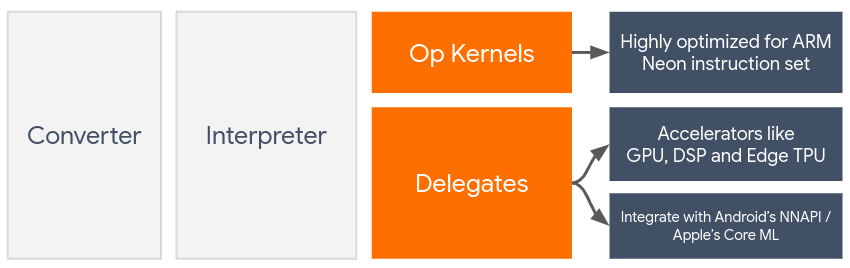
\includegraphics[width=0.8\textwidth]{Immagini/delegate_runtime.png}
    \caption{Distinzione tra kernel CPU e i delegati.}
    \label{fig:distinzione}
\end{figure}

\subsection{Scelta di un delegato}
TensorFlow Lite supporta più tipi di delegati, ognuno dei quali è ottimizzato per determinate piattaforme e particolari modelli. Nello specifico,
la scelta di un delegato si basa su due criteri principali: la piattaforma (Android o iOS) e il tipo di modello (a virgola mobile o quantizzato) da
accelerare. Per quanto riguarda la piattaforma:
\begin{itemize}
    \item Multipiattaforma (Android e iOS): GPU è l’unico tra i vari delegati che permette l’utilizzo sia su android che su iOS;
    \item Android: ci sono due delegati che supportano l’utilizzo su android (e NON su iOS), ossia il delegato NNAPI (disponibile in android 8.1 e
    versioni successive) e il delegato Hexagon (disponibile in versioni android precedenti che non supportano NNAPI);
    \item iOS: l’unico delegato ottimizzato per iOS è Core ML (disponibile su dispositivi mobili apple con SoC A12 o superiore).
\end{itemize}
Per quanto riguarda il tipo di modello:
\begin{center}
    \begin{tabular}{ |c|c|c|c|c| }
        \hline
        \textbf{Tipo di modello} & \textbf{GPU} & \textbf{NNAPI} & \textbf{Hexagon} & \textbf{CoreML} \\
        \hline
        Virgola mobile (32 bit) & \checkmark  & \checkmark & X & \checkmark \\
        \hline
        Quantizzazione float16 post-training & \checkmark & X & X & \checkmark \\
        \hline
        Quantizzazione della gamma dinamica post-training & \checkmark & \checkmark & X & X \\
        \hline
        Quantizzazione intera post-training & \checkmark & \checkmark & \checkmark & X \\
        \hline
        Training consapevole della quantizzazione & \checkmark & \checkmark & \checkmark & X \\
        \hline
        
    \end{tabular}
\end{center}
Ogni acceleratore è progettato per una certa larghezza di bit dei dati. Per esempio, se viene fornito un modello in virgola mobile ad un delegato che
supporta solo operazioni quantizzate a 8 bit (come il delegato Hexagon), allora il delegato non accetterà il modello il quale verrà eseguito interamente
sulla CPU.

Scegliere la configurazione di accelerazione hardware ottimale per il dispositivo di ciascun utente può essere difficile. Inoltre, abilitare la
configurazione errata su un dispositivo può causare elevata latenza, errori di runtime o problemi di precisione causati da incompatibilità hardware
sfociando, quindi, in un servizio scadente e insoddisfacente per l’utente. In questo contesto, TensorFlow Lite mette a disposizione un \textbf{servizio di
accelerazione per Android}: un'API che aiuta nella scelta della configurazione di accelerazione hardware ottimale per un determinato dispositivo utente e
per uno specifico modello, riducendo al minimo il rischio di errori di runtime o problemi di precisione.
Il servizio di accelerazione valuta diverse configurazioni di accelerazione sui dispositivi target eseguendo benchmark di inferenza con il modello
TensorFlow Lite creato. I risultati dell’esecuzione dei benchmark possono essere salvati su cache e utilizzati durante l’inferenza. Inoltre, questi
benchmark sono fuori processo, riducendo al minimo il rischio di arresti anomali dell’applicazione Android.
Fornendo il  modello, i campioni di dati e i risultati attesi il servizio di accelerazione eseguirà un benchmark di inferenza TFLite per fornire
consigli hardware allo sviluppatore.

\begin{figure}[ht]
    \centering
    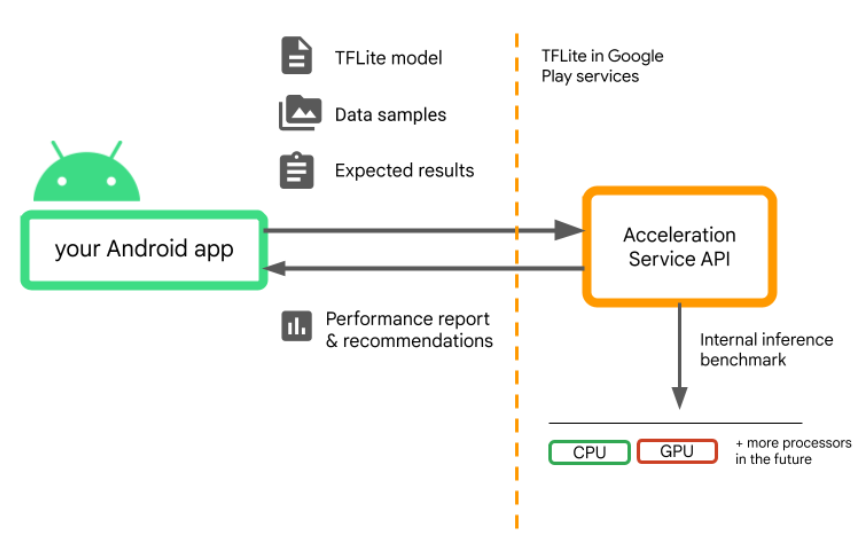
\includegraphics[width=0.6\textwidth]{Immagini/accelerazione.png}
    \caption{Schema riassuntivo del funzionamento del servizio di accelerazione}
    \label{fig:accelerazione}
\end{figure}


\subsection{Tools per la valutazione}
TensorFlow Lite fornisce strumenti di valutazione delle prestazioni e dell’accuratezza che consentono agli sviluppatori di analizzare e verificare
l’efficienza dell’utilizzo dei delegati nell’applicazione creata. I due principali tools utilizzati sono:
\begin{itemize}
    \item Tools per la latenza e l’utilizzo di memoria: stimano le prestazioni del modello considerando la latenza media di inferenza,
    l’overhead di inizializzazione, l’ingombro di memoria e altri;
    \item Tools per l’accuratezza e la correttezza: tendenzialmente, i delegati eseguono calcoli con una precisione differente rispetto ai kernel CPU.
    Di conseguenza, quando uso un delegato per l’accelerazione hardware la precisione tende a diminuire. Questo non succede sempre: per esempio la GPU,
    che esegue operazioni in virgola mobile, potrebbe migliorare leggermente la precisione. I tools che misurano questa metrica possono essere basati o
    meno sulla task specifica da valutare.
\end{itemize}

\section{TensorFlow Lite per Android}
TensorFlow Lite dispone di ambienti di esecuzione predefiniti e personalizzabili per l’esecuzione rapida e efficiente di modelli Android, incluse le opzioni per l'accelerazione hardware.

Come possiamo \textbf{eseguire un modello su Android}? Un modello TensorFlow Lite, all’interno di un’app Android, acquisisce ed elabora dati, generando una previsione basata sulla logica dello stesso modello.
Per essere eseguito, il modello ha bisogno di uno specifico ambiente di runtime e i dati di ingresso devono essere nel formato speciale tensor. Quando il modello esegue un’inferenza, produce risultati di
previsione nel formato tensor e li consegna all’app Android che, a seconda degli output ricevuti, intraprende una o più azioni (come mostrare a schermo il risultato o eseguire specifiche operazioni di calcolo).

\begin{figure}[ht]
    \centering
    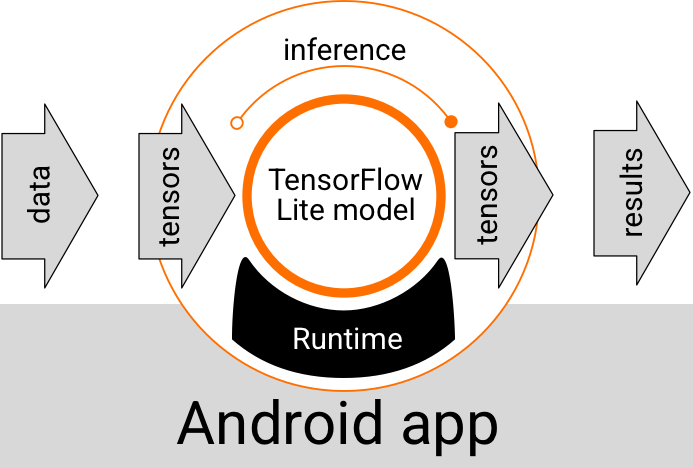
\includegraphics[width=0.6\textwidth]{Immagini/esecuzione.png}
    \caption{Schema di esecuzione di un modello in un app Android.}
    \label{fig:esecuzione}
\end{figure}

L’app, quindi, ha bisogno dei seguenti elementi per utilizzare un modello TF Lite:
\begin{itemize}
    \item Ambiente di runtime: per l’esecuzione del modello;
    \item Modellatore di input: per convertire i dati di ingresso nel formato textit{tensor};
    \item Modellatore di output: per ricevere i tensor di output e interpretarli come risultati di previsione.
\end{itemize}

\subsection{Ambiente di runtime}
Per l’esecuzione di un modello TensorFlow Lite su un app android c’è bisogno di un ambiente di runtime il quale può essere abilitato nei seguenti modi:
\begin{itemize}
    \item Google play services.
    \item Ambiente di runtime TensorFlow Lite Stand-alone.
\end{itemize}

Utilizzare i servizi Google Play è l’approccio preferito e consigliato. Infatti, questo ambiente di runtime è più efficiente in termini di spazio poiché si carica in modo dinamico, riducendo le dimensioni dell’app.
I servizi Google Play, inoltre, utilizzano automaticamente la versione più recente e aggiornata del runtime di TensorFlow Lite, offrendo funzionalità aggiuntive e prestazioni in continuo miglioramento. 
Adottare un ambiente di runtime fornito da Google Play Services ha degli svantaggi: il set di delegati per l’accelerazione hardware da cui si può scegliere si riduce e non sono supportate API TensorFLow Lite sperimentali
(come le operazioni personalizzate). Nel caso in cui i servizi Google Play non siano inclusi nell’app o nel caso in cui lo sviluppatore debba gestire il proprio modello machine learning “da vicino”, allora è conveniente usare
l’ambiente runtime TensorFlow Lite stand-alone che aggiunge codice nell’app, garantendo allo sviluppatore un maggiore controllo del runtime di machine learning al costo di un incremento della dimensione dell’app. 
Entrambi gli ambienti di runtime possono essere acceduti utilizzando specifiche API e librerie di sviluppo all’app.

\subsection{API e librerie di sviluppo}
Per integrare i modelli TensorFlow Lite in un applicazione Android, è possibile utilizzare due API molto utili fornite da TensorFlow Lite stesso:
\begin{itemize}
    \item L’API TensorFlow Lite Task;
    \item L’API TensorFLow LIte Interpreter.
\end{itemize}

Quali sono le differenze? L’API Interpreter fornisce classi e metodi per eseguire inferenze su modelli TensorFlow Lite già esistenti mentre L’API Task racchiude l’API Interpreter in un wrap che dispone di un’interfaccia
di programmazione ad alto livello per la gestione di attività di machine learning riguardo a dati visivi, audio e testuali. L’API Task viene sempre utilizzata nello sviluppo di applicazioni AI mobile, salvo casi specifici
in cui il dispositivo non è in grado di supportare tale API. Entrambe le API possono essere accedute tramite i servizi di Google Play.

\subsection{I tensori}
Al fine di comprendere maggiormente la prossima sezione, è giusto approfondire il concetto di tensore. Un tensore è un array multidimensionale con un tipo uniforme (chiamato dtype, o data type) di cui vettori, matrici, funzioni
lineari ed endomorfismi costituiscono casi particolari. Tutti i tensori sono immutabili: non è mai possibile modificare il contenuto di un tensore, solamente crearne uno nuovo (a eccezione del caso specifico dei tensori di tipo tf.Variable).
Oltre al data type, i tensori possiedono due caratteristiche principali: la forma (o shape), ossia la lunghezza di ogni dimensione, e il grado (o rank) che consiste nel numero di dimensioni del tensore e può essere considerato
il suo ordine di grandezza.

Per esempio, uno scalare è un tensore di rank 0 e di shape nulla, un vettore è un tensore di rank 1 e di shape che corrisponde al numero di elementi del vettore, una matrice è un tensore di rank 2 (2 dimensioni) e di shape costituita
da due numeri: il numero di righe e il numero di colonne.

Al fine di creare un rete neurale, si utilizzano delle rappresentazioni grafiche per mostrare il flusso di calcolo dei dati e le operazioni avvenute. Per fare ciò, si utilizza un grafo: la rappresentazione, per mezzo di nodi,
di operazioni eseguite sui tensori. Il grafo è costituito da nodi che rappresentano i tensori e i dati memorizzati all’interno di essi e da nodi che rappresentano le operazioni su tali dati. I tensori si uniscono tra di loro
per formare unità neurali più complesse, come il percettrone.

Una rete neurale è costituita da innumerevoli percettroni, caratterizzando la complessità del mondo AI. Dopo questa brevissima introduzione dei tensori, torniamo a TensorFlow Lite che, come suggerisce il nome, sfrutta a pieno
la struttura dati appena introdotta.

\begin{figure}[ht]
    \centering
    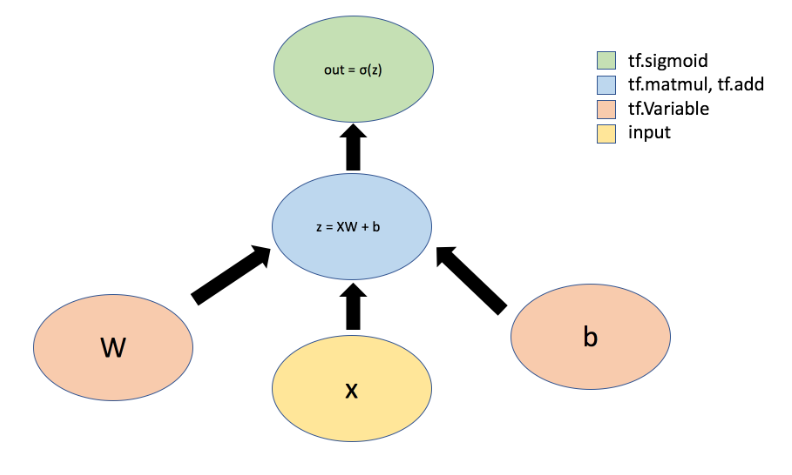
\includegraphics[width=0.7\textwidth]{Immagini/tensore.png}
    \caption{Percettrone, esempio di un semplice grafo con tensori e operazioni}
    \label{fig:tensore}
\end{figure}

\newpage
\section{Gestione dei dati in input}
Come già anticipato, per elaborare i dati di input è necessario che essi siano nel formato di tensore. Il tensore, inoltre, deve essere in una specifica forma. Ogni modello TensorFlow Lite di machine learning, quindi, deve trasformare
un dato in input dal suo formato nativo (immagine, testo, audio…) in un tensore con la specifica forma richiesta dal modello. Molto spesso il formato richiesto viene specificato nei metadati del modello. Come eseguire tale trasformazione?
TensorFlow Lite fornisce una libreria apposita chiamata TensorFlow Lite Task che dispone di una logica di gestione dati per la conversione dei dati da un qualsiasi formato a un tensore con la forma giusta.

Una volta ottenuto un ambiente di runtime ottimale, un modello e dei dati di input nel formato richiesto è possibile eseguire inferenze come descritto precedentemente nel report.

\section{Gestione dei risultati in output}
Eseguita l’inferenza, il modello produce in output dei risultati nella forma di tensori che devono essere gestiti ed interpretati dall’applicazione android agendo o mostrando a schermo un risultato per l’utente. 
I tensori di output possono essere dei semplici numeri che corrispondono ad un singolo risultato (per esempio, 0 = gatto, 1 = cane, 2 = pesce) per una classificazione di immagini, ma possono essere anche risultati estremamente
complessi come diversi riquadri di delimitazione nel caso in cui vi siano più oggetti classificati in un’immagine, insieme a delle valutazioni di affidabilità delle previsioni nell’intervallo [0, 1].

Molto spesso la descrizione dei risultati di output e di come interpretarli viene fornita dai metadati incorporati nel modello.

\section{Approcci di sviluppo avanzati}
Nel caso in cui vengano utilizzati modelli TensorFlow Lite più sofisticati, potrebbe essere necessario utilizzare percorsi di sviluppo avanzati e più complicati rispetto a quanto descritto sopra. Quindi,
si utilizzano delle tecniche avanzate per sviluppare ed eseguire modelli TensorFlow LIte in un’app Android:
\begin{itemize}
    \item Ambiente di runtime avanzato: quando si dispone di un modello di machine learning che utilizza operazioni non supportate dall’ambiente di runtime standard di TensorFlow Lite o da quello fornito dai servizi di Google Play,
    è possibile utilizzare degli ambienti runtime avanzati: l’ambiente runtime TensorFlow Lite Flex, che permette di implementare operatori specifici per il proprio modello el’ ambiente runtime TensorFlow Lite personalizzato.
    Come opzione ancora più avanzata, è possibile importare la libreria TensorFlow Lite su Android per l’inclusione di funzionalità e operatori richiesti per eseguire il proprio modello.
    \item APIs di C e C++: TensorFlow Lite fornisce delle API per eseguire modelli usando C e C++. L’utilizzo di queste API è consigliato quando l’applicazione usa Android NDK o se si vuole condividere codice tra piattaforme.
    \item Esecuzione del modello su un server: l’esecuzione dei modelli nella propria app Android permette di abbassare la latenza e migliorare la privacy per gli utenti. In alcuni casi, però, conviene eseguire il proprio modello
    su un server cloud: per esempio, questo approccio è consigliato se il modello è troppo grande e non è facilmente comprimibile in una dimensione gestibile da dispositivi Android degli utenti. Inoltre, si utilizza questa tecnica
    quando è prioritario garantire una performance consistente del modello su un vasto range di dispositivi.
    \item Ottimizzazione di modelli personalizzati: è importante considerare di ottimizzare il proprio modello personalizzato per ridurre costi di elaborazione e di memoria. L’approccio consigliato è sempre quello della quantizzazione. 
\end{itemize}
